\documentclass{VUMIFPSbakalaurinis}
\usepackage{algorithmicx}
\usepackage{algorithm}
\usepackage{algpseudocode}
\usepackage{amsfonts}
\usepackage{amsmath}
\usepackage{bm}
\usepackage{caption}
\usepackage{color}
\usepackage{float}
\usepackage{graphicx}
\usepackage{listings}
\usepackage{subfig}
\usepackage{url}
\usepackage{wrapfig}
\usepackage[table,xcdraw]{xcolor}
\usepackage[backend=biber]{biblatex}
\usepackage{enumitem}\setlist{nosep}
\usepackage{listings}
\usepackage{color}

\definecolor{codegreen}{rgb}{0,0.6,0}
\definecolor{codegray}{rgb}{0.5,0.5,0.5}
\definecolor{codepurple}{rgb}{0.58,0,0.82}
\definecolor{backcolour}{rgb}{0.95,0.95,0.92}

\lstdefinestyle{mystyle}{
	backgroundcolor=\color{backcolour},   
	commentstyle=\color{codegreen},
	keywordstyle=\color{magenta},
	numberstyle=\tiny\color{codegray},
	stringstyle=\color{codepurple},
	basicstyle=\footnotesize,
	breakatwhitespace=false,         
	breaklines=true,                 
	captionpos=b,                    
	keepspaces=true,                 
	numbers=left,                    
	numbersep=5pt,                  
	showspaces=false,                
	showstringspaces=false,
	showtabs=false,                  
	tabsize=2
}

\lstset{style=mystyle}

% Titulinio aprašas
\university{Vilniaus universitetas}
\faculty{Informatikos Institutas}
\department{Programų sistemų katedra}
%\papertype{Bakalauro darbas}
\papertype{Bakalauro darbas}
\title{Anomalijų aptikimas interneto prieigos stebėsenos sistemos įrašuose}
\titleineng{Detection of anomalies in internet access monitoring system data}
\author{Jokūbas Rusakevičius}
\supervisor{asist. dr. Vytautas Valaitis}
\reviewer{j. asist. Linas Petkevičius}
\date{Vilnius – \the\year}

% Nustatymai
\setmainfont{Palemonas}  
\bibliography{bibliografija}

\begin{document}
\maketitle

\setcounter{page}{2}

\sectionnonumnocontent{Santrauka}
TODO: Santrauka
% Nurodomi iki 5 svarbiausių temos raktinių žodžių (terminų).
% Vienas terminas gali susidėti iš kelių žodžių.
\raktiniaizodziai{raktinis žodis 1, raktinis žodis 2, raktinis žodis 3, raktinis žodis 4, raktinis žodis 5}   

\sectionnonumnocontent{Summary}
TODO: summary
\keywords{keyword 1, keyword 2, keyword 3, keyword 4, keyword 5}

\tableofcontents

\sectionnonum{Įvadas}
Šis darbas yra Programų Sistemų studijų baigiamasis bakalauro darbas apie anomalijų aptikimą interneto prieigos stebėsenos sistemos įrašuose naudojant „MacroBase“ atviro kodo analitinį įrankį bei „SQL“ paketą.

\subsectionnonum{Problematika}
Informacijos rinkimas fizine forma, juos užrašant ant popieriaus lapo, pasak MIT Media Lab direktoriaus Joi Ito, dar visai neseniai buvo vienintelis būdas rinkti, klasifikuoti ir saugoti duomenis. Žmogus mintis ir idėjas užrašydamas ant popieriaus lapo – paversdavo žiniomis (angl. \textit{knowledge}). Tačiau laikai keičiasi, ir dabartinė didžiųjų duomenų situacija kinta. Dėl milžiniškų surenkamų duomenų kiekio, nėra trivialu atskirti naudingus ir nenaudingus duomenis, todėl, natūraliai, negalima visų surenkamų duomenų automatiškai priskirti prie ir vadinti žiniomis. Surinkti duomenys nėra žinios, kol jų nepradedama nagrinėti, analizuoti ir filtruoti, ir tik pradėjus šį procesą galima pastebėti, kad gaunama informacija yra įdomi ir netgi svarbi \cite{movie}.\par
Duomenų, kuriais yra operuojama, juos yra renkama ir saugoma, kiekiai nuolatos didėja \cite{iot}. Iš tiesų, dėl daugelio priežasčių net greitis, kuriuo šie duomenys yra generuojami eksponentiškai kyla \cite{zettabytes}. Jau 2015–2016 metais didžiosios socialinių tinklų kompanijos Twitter, Facebook ir LinkedIn pranešė fiksuojančios iki 12 milijonų įvykių (angl. \textit{events}) per sekundę \cite{twitter, facebook, linkedin}. Šie duomenų kiekiai gerokai lenkia žmogaus gebėjimą juos apdoroti bei žymiai apsunkina darbą tiek analitikams, tiek analitiniams įrankiams. Keli iš geriausių (angl. \textit{best-of-class}) šių dienų taikomųjų programų operatorių praneša panaudojantys anekdotiškai mažą jų surenkamų duomenų kiekį – mažiau nei 6\% \cite{prioritizing_attention}.




\section{Duomenų analizės eksperimentas naudojant „MacroBase SQL“ modulį}

\subsection{Duomenų rinkinys}
Šiame skyriuje aprašyti eksperimentui pritaikyti IPSS duomenų rinkiniai.

\subsubsection{Eksperimentui pritaikyti duomenys}
Eksperimentui buvo naudojami Lietuvos Respublikos ryšių reguliavimo tarnybos administruojamos Interneto prieigos stebėsenos sistemos (IPSS) atliekami belaidės interneto prieigos duomenų perdavimo spartos kontrolinių matavimų 2014–2018 metų rezultatai. Matavimai atlikti operatorių UAB „Bitė Lietuva“, AB „Telia Lietuva“, UAB „TELE2“ ir AB Lietuvos radijo ir televizijos centro (LRTC) judriojo ryšio tinkluose visoje Lietuvos teritorijoje. Matavimų paskirtis yra stebėti ir įvertinti teikiamų interneto prieigos paslaugų kokybę, kaip to reikalauja Europos Sąjungos direktyvos, taip pat supažindinti visuomenę su tokių matavimų rezultatais. Įrašai pateikiami CSV formato failais. Iš viso gauti 3 failai skirti trims skirtingoms technologijoms: 3G, LTRE ir WiMAX. Viename CSV faile priklausomai nuo failui priskirtos technologijos buvo apytiksliai 136000, 157000 ir 18000 įrašų eilučių, vidutiniškai 104000. Vieno failo dydis vidutiniškai 8,5MB.

\subsubsubsection{Duomenų aprašymas}
Kiekvienas IPSS įrašų failas prasideda antraštės (angl. \textit{header}) eilute, kuri susideda iš faile saugomų įrašų sąrašo laukų (angl. \textit{fields}) pavadinimų. IPSS įrašų sarašų laukai ir jų paaiškinimas:

\begin{itemize}
	\item \textbf{Bendri visiems failams laukai:}
		\subitem \textbf{Data ir laikas} – matavimo įrašo fiksavimo data ir laikas, užrašoma „yyyy-MM-dd hh:mm:ss“ formatu.
		\subitem \textbf{Platuma} – matavimo įrašo fiksavimo koordinačių platuma užrašoma dešimtainiais laipsniais (angl. \textit{decimal degrees}).
		\subitem \textbf{Ilguma} – matavimo įrašo fiksavimo koordinačių ilguma užrašoma dešimtainiais laipsniais (angl. \textit{decimal degrees}).
		\subitem \textbf{Operatorius} – matavimo įrašo operatoriaus skaitinis kodas arba pavadinimas (vieno iš jau minėtų operatorių: „Bitė Lietuva“, „Telia Lietuva“, „TELE2“ ir LRTC).
		\subitem \textbf{RSSI} – signalo stiprumo indikatorius (angl. \textit{received signal strength indicator}).
		\subitem \textbf{Sparta kbit/s} – sveikuoju skaičiumi nurodomas užfiksuotas matavimo greitis kilobitais per sekundę.
	\item \textbf{3G failui išskirtiniai laukai:}
		\subitem \textbf{Celės id} – matavimą atlikusio įrenginio identifikacijos kodas.
		\subitem \textbf{Ryšio tinklas} – nurodo matuojamo ryšio tinklą (visi įrašai šiame faile ryšio tinklo lauke turi reikšmę „3G“).
		\subitem \textbf{3G ryšio technologija} – nurodo matavimo metu naudotą ryšio technologiją (vieną iš: „DC-HSPA+“, „HSDPA“, „HSPA“, „HSPA+“, „HSUPA“ arba „WCDMA“).
	\item \textbf{LTE failui išskirtiniai laukai:}
		\subitem \textbf{Celės id} – matavimą atlikusio įrenginio identifikacijos kodas.
		\subitem \textbf{RSRP} – angl. \textit{reference signals received power} panašiai kaip RSSI signalo stiprumo identifikatorius LTE tinklams.
		\subitem \textbf{RSRQ} – angl. \textit{reference signals received quality} signalo kokybės laukas (šiame dokumente šis laukas reikšmės neturi – „NULL“)).
		\subitem \textbf{SINR} – signalo ir trukdžių bei triukšmo santykis (angl. \textit{signal-to-interference-plus-noise ratio}) (šiame dokumente šis laukas reikšmės neturi – „NULL“)).
		\subitem \textbf{Ryšio tinklas} – nurodo matuojamo ryšio tinklą (visi įrašai šiame faile ryšio tinklo lauke turi reikšmę „LTE“).
	\item \textbf{WiMAX failui išskirtiniai laukai:}
		\subitem \textbf{Bazinės stoties id} – matavimą atlikusios stotelės MAC adresas.
		\subitem \textbf{CINR} – trikdžių ir triukšmo santykis (angl. \textit{carrier to interference-plus-noise ratio}).
		\subitem \textbf{Ryšio technologija} – nurodo matuojamo ryšio tinklą (visi įrašai šiame faile ryšio technologijos lauke turi reikšmę „WIMAX“).
\end{itemize}
IPSS matavimai atliekami automobilyje sumontuotos įrangos, todėl jie neapima viso Lietuvos ploto, tik pagrindinius kelius, geležinkelius ir miestus. Atliktų matavimų koordinates galima pamatyti \ref{img:3G-0}, \ref{img:LTE-0} ir \ref{img:WiMAX-0} pav.
\begin{figure}[H]
	\centering
	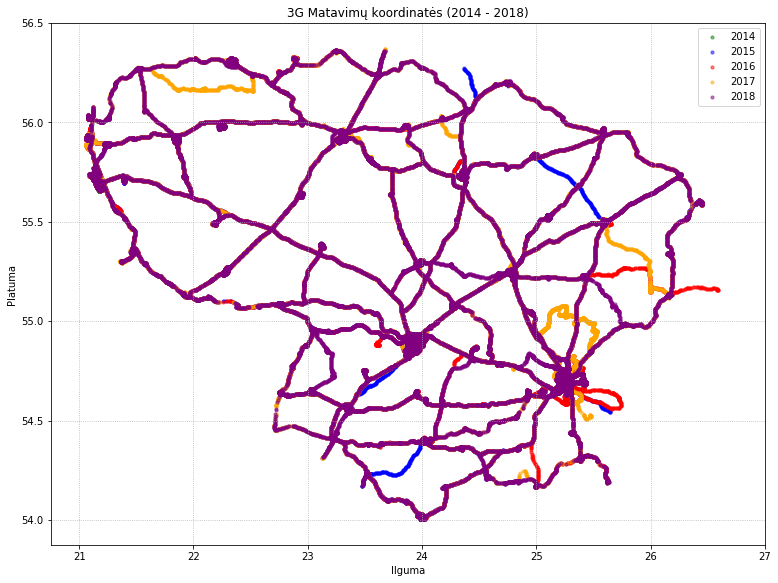
\includegraphics[scale=0.5]{img/3G-0}
	\caption{3G Matavimai 2014–2018 metais}
	\label{img:3G-0}
\end{figure}
\begin{figure}[H]
	\centering
	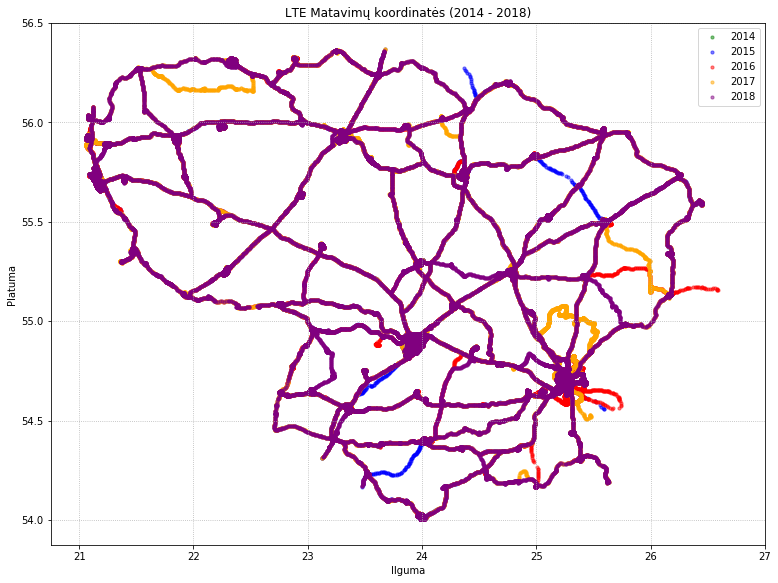
\includegraphics[scale=0.5]{img/LTE-0}
	\caption{LTE Matavimai 2014–2018 metais}
	\label{img:LTE-0}
\end{figure}
\begin{figure}[H]
	\centering
	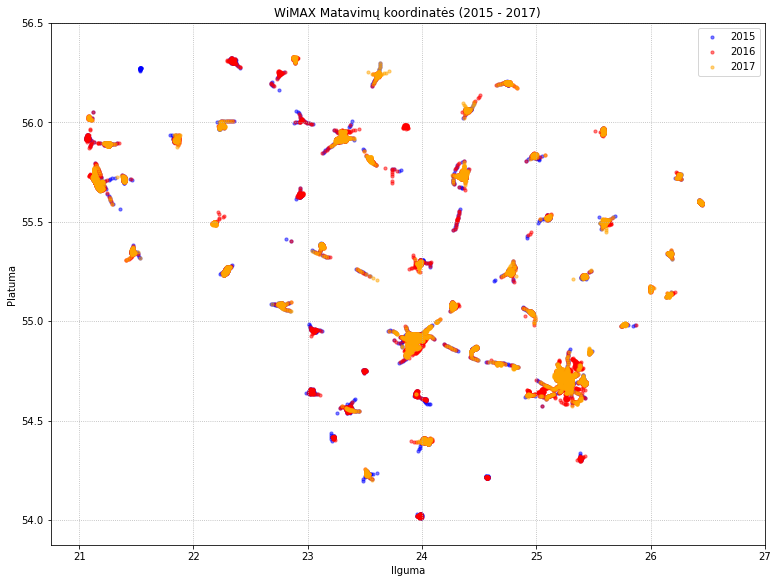
\includegraphics[scale=0.5]{img/WiMAX-0}
	\caption{WiMAX Matavimai 2015–2017 metais}
	\label{img:WiMAX-0}
\end{figure}
Aiškiau išskirtus įrašų koordinačių duomenis galima rasti Priede \ref{coordpav}.


\subsubsubsection{Duomenų paruošimas}
Eksperimentui atlikti buvo atrinkti laukai, kurie turi reikšmes visose įrašų sąrašo eilutėse bei taip pat buvo atmesti pasikartojančios informacijos laukai (ryšio tinklo ir ryšio technologijos laukai, kurie nurodo, koks tinklo tipas iš trijų tiriamųjų yra naudojamas faile). Taip pat buvo nuspręsta datos ir laiko lauką pakeisti tik metų lauku. Taigi, 3G tinklui atrinkti šie pradiniai laukai: metai, ilguma, platuma, operatorius, celės id, rssi, 3G ryšio technologija ir sparta; iš LTE duomenų atrinkti laukai: metai, ilguma, platuma, operatorius, celės id, rssi, rsrp, sparta; iš WiMAX duomenų atrinkti laukai: metai, ilguma, platuma, operatorius, bazinės stoties id, rssi, cirn, sparta.\par
Eksperimentui atlikti buvo reikalingas CSV formato failai, kuriuose nebūtų lietuviškų raidžių ir būtų naudojami vieno žodžio arba vienos simbolių eilutės antraštės pavadinimai (pavyzdžiui, tarpai gali būti pakeičiami „\_“ simboliu), todėl buvo realizuoti „Python“ skriptas, kuris nuskaito duotųjų duomenų CSV failus ir juos apdorojus, grąžina naujus CSV failus. Skriptas kurtas ir leistas „Jupyter Notebook“ aplinkoje. Skripte galima pasirinkti kelią iki duotųjų CSV failų ir kelią iki naujai sukuriamų CSV failų. Šis skriptas skirtas pervadinti antraštes, atskirti metus ir atrinkti nereikalingus laukus. Skriptai atlieka šiuos veiksmus 3 kartus kiekvienai ryšio technologijai (3G, LTE, WiMAX) (Priedas \ref{script1}):
\begin{enumerate}
	\item Nuskaito CSV įrašų failą pateiktą nurodytu keliu.
	\item Sukuria naują CSV failą nurodytų keliu ir pavadinimu.
	\item Įrašo į naujai sukurtą CSV failą, naują antraštę, su naujais angliškais vieno žodžio (simbolių eilutės) pavadinimais.
	\item Vykdo ciklą, kuris skaitant po vieną eilutę iš pradinio failo įrašo tik reikalingus duomenis į naują failą bei iš datos ir laiko paima tik metus. Taip pat kiekviena eilutė yra skaičiuojama.
	\item Išvedamas galutinis eilučių skaičius.
\end{enumerate}
Atrinkus duomenis iš pradinių duomenų buvo sukurtas antras skriptas skirtas išgauti daugiau informacijos iš koordinačių. Kadangi ilgumos ir platumos laukai yra realiosios reikšmės, jomis yra nepatogu naudotis. Tam buvo sukurtas dar vienas skriptas, kuris suapvalina koordinačių laukus iki pasirinkto skaičiaus po kableliu taip sumažinant unikalių reikšmių kiekį. Šios reikšmės buvo pridėtos į joms sukurtus naujus laukus. Papildomai originalios koordinačių reikšmės buvo panaudotos išgauti kiekvieno koordinačių taško aukštį virš jūros lygio. Ši bei suapvalinta iki dešimčių metrų reikšmės buvo pridėtos į papildomus joms sukurtus laukus. Taigi naujas „Python“ skriptas nuskaito prieš tai sukurtus CSV failus, gauna aukščio virš jūros lygio reikšmes, suapvalina koordinačių bei aukščio reikšmes ir sukuria naujus CSV failus pasirinktu adresu. Skriptai atlieka šiuos veiksmus 3 kartus kiekvienai ryšio technologijai (3G, LTE, WiMAX) (Priedas \ref{script2}):
\begin{enumerate}
	\item Nuskaito CSV įrašų failą pateiktą nurodytu keliu.
	\item Iš nuskaitytų duomenų atskiriama antraštė nuo įrašų.
	\item Iš antraštės surandami metų, platumos ir ilgumos laukų indeksai.
	\item Pasinaudojus gautais indeksais, sukuriami visų ilgumos ir platumos reikšmių masyvai.
	\item Vykdomas ciklas, kuris visus įrašus padalina į pasirinkto žingsnio dydžio dalis.
	\item Vykdomas ciklas cikle, kuris visas ilgumos ir platumos reikšmes sujungia į „string“ tipo kintamuosius, kuriuose ilguma ir platuma yra atskirtos kableliu „,“.
	\item Kiekvienam žingsniui, iš platumos ir ilgumos bendrų kintamųjų sukuriamas vienas „string“ kintamasis, kur kiekvienas bendras koordinačių kintamasis yra atskirtas vertikaliu brūkšniu „|“.
	\item Vykdomas ciklas, kuris kiekvienai žingsnio koordinačių kiekio „string“ kintamajam sukuria URL užklausą „Jawg.io“ API, kuri susideda iš koordinačių kintamojo, pagrindinio URL ir vartotojo prieigos žymės (angl. \textit{access token}).
	\item Kiekvienam žingsniui yra siunčiama HTTP užklausa, kuri grąžina JSON duomenų struktūrą su koordinatėmis ir jų aukščiais virš jūros lygio.
	\item Iš JSON duomenų struktūros atskiriamos aukščio virš jūros lygio reikšmės ir jos yra patalpinamos į masyvą atitinkamu indeksu.
	\item Vykdomas ciklas, kuris kiekvienam nuskaitytam įrašui sukuria nauja įrašą su suapvalintomis iki pasirinkto skaičiaus po kablelio reikšmėmis bei aukščio virš jūros lygio ir suapvalinta iki dešimčių aukščio virš jūros lygio reikšmėmis. Šie įrašai sujungiami su atitinkamais įrašais ir sukuriamas naujas masyvas su šiais įrašais.
	\item Sukuriamas naujas CSV failas nurodytu keliu ir pavadinimu.
	\item Įrašoma nauja antraštė su papildytais pavadinimais.
	\item Vykdomas ciklas, kuris kiekvieną naujai papildytą įrašą įveda į naują CSV failą.
\end{enumerate}
Eksperimentui atlikti buvo nuskaityti ir apdoroti apie 300000 įrašų, vidutiniškai 100000 per failą.
TODO: pridėti citatą
\subsection{Eksperimento aplinkos paruošimas}
Eksperimentas buvo atliekamas naudojant „Ubuntu (64-bit)“ operacinę sistemą įdiegtą virtualioje mašinoje „Oracle VM VirtualBox“. „MacroBase SQL“ įdiegtas ir paruoštas darbui naudojantis „MacroBase“ dokumentacija.

\subsubsection{Virtuali mašina eksperimentui}
„MacroBase“ pateikiami pavyzdžiai ir konfigūraciniai nurodymai yra pateikiami „Linux“ operacinėms sistemoms. Dėl šios priežasties, eksperimentui atlikti buvo pasirinkta atviro kodo nemokama operacinė sistema „Ubuntu“. Dėl paprastumo buvo nuspręsta naudoti virtualią mašiną operacinei sistemai įdiegti. Atviro kodo nemokama virtuali mašina „Oracle VM VirtualBox“ buvo pasirinkta šiai užduočiai. Galutinės eksperimentui naudotos sisteminės specifikacijos:
\begin{itemize}
	\item Reali mašina, kurioje atliekamas eksperimentas – nešiojamasis kompiuteris „Lenovo Y50-70“.
		\subitem Realios mašinos Operacinė sistema \textbf{„Microsoft Windows 10 Pro“}, versija	10.0.17763.
		\subitem Realios mašinos procesorius: \textbf{i7-4720HQ}
		\subitem Realios mašinos operatyvioji atmintis: \textbf{8GB}
	\item \textbf{„Oracle VM VirtualBOX“} virtuali mašina, versija  \textbf{6.0.8} r130520 (Qt5.6.2).
		\subitem Virtualios mašinos operacinės sistemos „Ubuntu“ 64 bitų versiją \textbf{„Ubuntu (64-bit)“}, versija \textbf{18.04 LTS}.
		\subitem Virtualiai mašinai suteiktas virtualus standusis diskas: \textbf{40GB}.
		\subitem Virtualiai mašinai skirta operatyvioji atmintis: \textbf{4GB}.
\end{itemize}

\subsubsubsection{Virtualios mašinos paruošimas}
Virtualios mašinos paruošimas eksperimentui:
\begin{enumerate}
	\item Iš „Oracle VM VirtualBox“ internetinės svetainės atsisiųstas naujausias „Windows 10“ operacinei sistemai skirtas diegimo failas (\url{https://www.virtualbox.org/wiki/Downloads}).
	\item Sekant sąrankos vedlio nurodymus įdiegta „Oracle VM VirtualBox“ virtuali mašina.
	\item Iš „Ubuntu“ internetinės svetainės atsisiųstas naujausias „Ubuntu (64-bit)“ operacinės sistemos ISO failas (\url{https://www.ubuntu.com/download/desktop}).
	\item Atidarius „Oracle VM VirtualBox“ programinę įrangą pradėtas naujos virtualios mašinos pridėjimo procesas spaudžiant mygtuką su tekstu „New“.
	\item Sekant naujos virtualios mašinos pridėjimo langus pasirinktos šios parinktys:
		\subitem Operacinės sistemos tipas: „Linux“.
		\subitem Versija: „Ubuntu (64-bit)“.
		\subitem Operatyviosios atminties kiekis megabaitais: 4096MB.
		\subitem Virtualus standusis diskas: 40GB.
	\item „Oracle VM VirtualBox“ pagrindiniame lange pasirinkus naujai sukurtą vitualią mašiną spaustas mygtukas su tekstu „Start“.
	\item Atidarytame virtualios mašinos lange pasirinktas anksčiau atsiųstas „Ubuntu (64-bit)“ ISO failas.
	\item Pasirinkta „Install“ operacija ir sekant diegimo vedlį, įdiegta „Ubuntu (64-bit)“ operacinė sistema.	
\end{enumerate}

\subsubsection{„MacroBase“ analitinio įrankio paruošimas}
„MacroBase SQL“ diegiamas pagal „MacroBase“ dokumentacijoje nurodytus žingsnius. Tačiau prieš pradedant diegimo procesą reikia įdiegti įrankius bei papildomus paketus, tam kad „MacroBase“ taisyklingai veiktų bei būtų galima atlikti diegimo procesą. Eksperimentui naudotos programinės įrangos specifikacijos:
\begin{itemize}
	\item „MacroBase“ versija v1.0.
	\item Java JRE versija 1.8.0\_212.
	\item Java JDK versija 1.8.0\_212.
	\item „Apache Maven“ versija 3.6.0.
\end{itemize}

\subsubsubsection{„MacroBase SQL“ diegimui reikalingi papildomi paketai}
Sėkmingam „MacroBase SQL“ diegimo procesui naujai paruoštoje „švarioje“ „Ubuntu“ operacinėje sistemoje, reikalingi papildomi pagalbiniai paketai. Šiuos paketus įdiegti buvo naudojamos šios terminalo komandos:
\begin{enumerate}
	\item Versijavimo kontrolės sistemos „Git“ diegimas:
	\begin{verbatim}
	sudo apt install git
	\end{verbatim}
	\item Java projektų valdymo ir diegimo priemonės „Apache Maven“ diegimas:
	\begin{verbatim}
	sudo apt install maven
	\end{verbatim}
	\item Java JRE diegimas:
	\begin{verbatim}
	sudo apt install openjdk-8-jre
	\end{verbatim}
	\item Java JDK diegimas:
	\begin{verbatim}
	sudo apt install openjdk-8-jdk
	\end{verbatim}
\end{enumerate}

\subsubsubsection{„MacroBase SQL“ analitinio įrankio diegimas}
Sekant „MacroBase“ dokumentacijoje nurodytus žingsnius įdiegtas „MacroBase SQL“ įrankis:
\begin{enumerate}
	\item Atidarytas „Ubuntu“ terminalas.
	\item Klonuota projekto repozitorija:
	\begin{verbatim}
	git clone https://github.com/stanford-futuredata/macrobase.git
	\end{verbatim}
	\item Pereita į „MacroBase“ naujai sukurtą direktoriją:
	\begin{verbatim}
	cd macrobase
	\end{verbatim}
	\item Paleistas „MacroBase SQL“ kompiliavimo ir paruošimo BASH skriptas:
	\begin{verbatim}
	./build.sh sql
	\end{verbatim}
	\item Patikrinta ar diegimas atliktas teisingai ir „MacroBase SQL“ įrankis veikia korektiškai pasinaudojus demonstraciniais duomenimis:
	\begin{verbatim}
	bin/macrobase-sql -f sql/demo.sql
	\end{verbatim}
\end{enumerate}

\subsection{Eksperimento vykdymo eiga}
Šiame poskyryje aprašoma eksperimento vykdymo eiga naudojant IPSS pateiktus 2014-2018 metų duomenų rinkinius naudojantis „MacroBase SQL“ analitinį įrankį.

\subsubsection{Konfiguracija}
„MacroBase SQL“ paleidimui buvo naudojama komandinė eilutė, kuriai paduodami SQL formato failai. Šiuose failuose nurodomi tokia informacija:
\begin{itemize}
	\item 
\end{itemize}

\subsubsection{Eksperimento eiga}
Šiame skyriuje aprašyta eksperimento eiga 








\sectionnonum{Rezultatai ir išvados}
Rezultatų ir išvadų dalyje išdėstomi pagrindiniai darbo rezultatai (kažkas
išanalizuota, kažkas sukurta, kažkas įdiegta), toliau pateikiamos išvados
(daromi nagrinėtų problemų sprendimo metodų palyginimai, siūlomos
rekomendacijos, akcentuojamos naujovės). Rezultatai ir išvados pateikiami
sunumeruotų (gali būti hierarchiniai) sąrašų pavidalu. Darbo rezultatai turi
atitikti darbo tikslą.

\printbibliography[heading=bibintoc]  % Šaltinių sąraše nurodoma panaudota
% literatūra, kitokie šaltiniai. Abėcėlės tvarka išdėstomi darbe panaudotų
% (cituotų, perfrazuotų ar bent paminėtų) mokslo leidinių, kitokių publikacijų
% bibliografiniai aprašai. Šaltinių sąrašas spausdinamas iš naujo puslapio.
% Aprašai pateikiami netransliteruoti. Šaltinių sąraše negali būti tokių
% šaltinių, kurie nebuvo paminėti tekste. Šaltinių sąraše rekomenduojame
% necituoti savo kursinio darbo, nes tai nėra oficialus literatūros šaltinis.
% Jei tokių nuorodų reikia, pateikti jas tekste.

% \sectionnonum{Sąvokų apibrėžimai}
\sectionnonum{Santrumpos}
\begin{itemize}
	\item CSV
	\item 3G
	\item LTE
	\item MAC adresas
	\item IPSS
	\item URL
	\item API
	\item HTTP
	\item JSON
	\item JRE
	\item JDK
	\item BASH
	\item SQL
\end{itemize}
Sąvokų apibrėžimai ir santrumpų sąrašas sudaromas tada, kai darbo tekste
vartojami specialūs paaiškinimo reikalaujantys terminai ir rečiau sutinkamos
santrumpos.

\appendix  % Priedai
% Prieduose gali būti pateikiama pagalbinė, ypač darbo autoriaus savarankiškai
% parengta, medžiaga. Savarankiški priedai gali būti pateikiami ir
% kompaktiniame diske. Priedai taip pat numeruojami ir vadinami. Darbo tekstas
% su priedais susiejamas nuorodomis.

\section{IPSS matavimų koordinatės 2014–2018 metais} \label{coordpav}
IPSS \textbf{3G} ryšio technologijos matavimai 2014–2018 metais. Viso 136003 įrašai.
\begin{figure}[H]
	\centering
	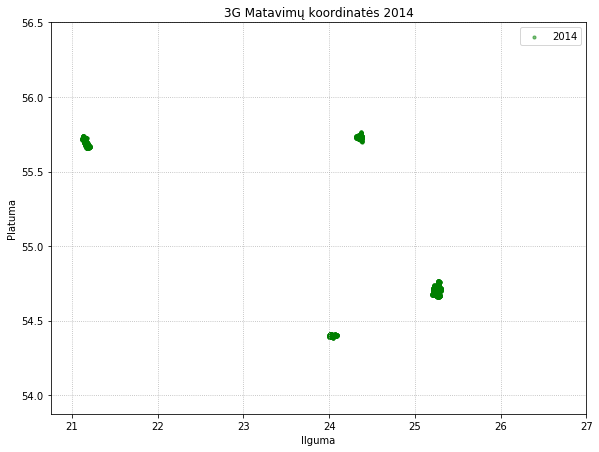
\includegraphics[scale=0.33]{img/3G-1}
	\caption{3G Matavimai 2014 metais. Viso – 2245 matavimai}
	\label{img:3G-1}
\end{figure}
\begin{figure}[H]
	\centering
	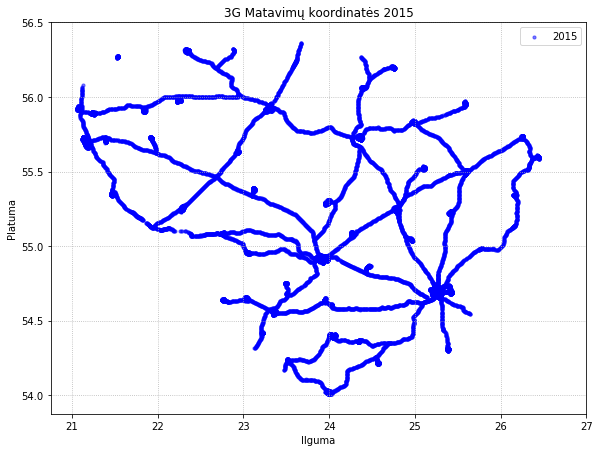
\includegraphics[scale=0.33]{img/3G-2}
	\caption{3G Matavimai 2015 metais. Viso – 19427 matavimai}
	\label{img:3G-2}
\end{figure}
\begin{figure}[H]
	\centering
	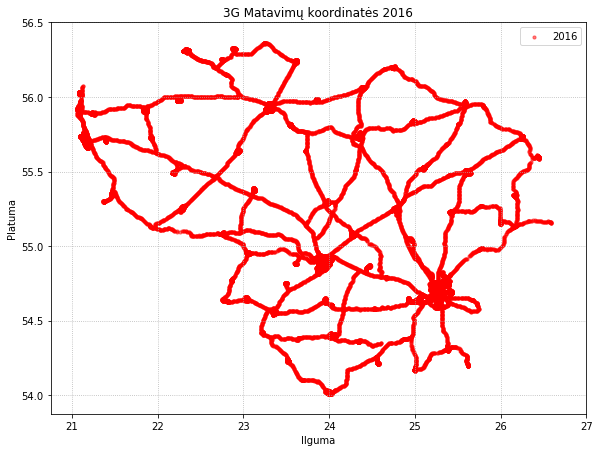
\includegraphics[scale=0.33]{img/3G-3}
	\caption{3G Matavimai 2016 metais. Viso – 34769 matavimai}
	\label{img:3G-3}
\end{figure}
\begin{figure}[H]
	\centering
	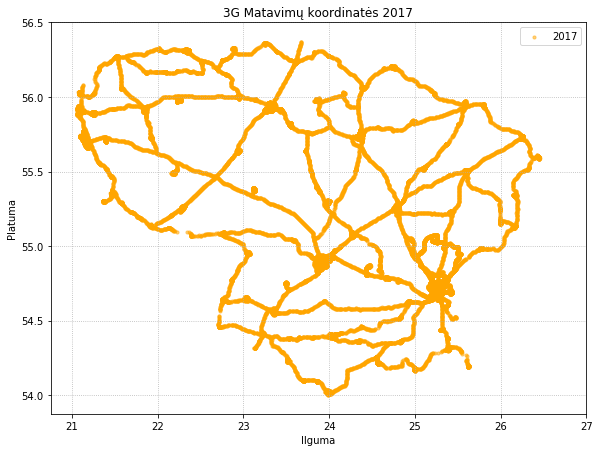
\includegraphics[scale=0.33]{img/3G-4}
	\caption{3G Matavimai 2017 metais. Viso – 38789 matavimai}
	\label{img:3G-4}
\end{figure}
\begin{figure}[H]
	\centering
	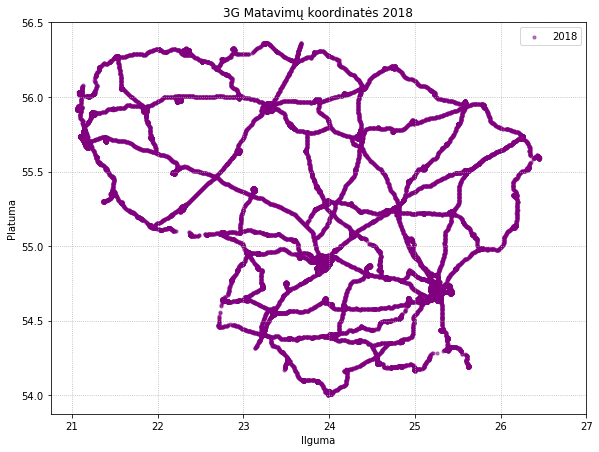
\includegraphics[scale=0.33]{img/3G-5}
	\caption{3G Matavimai 2018 metais. Viso – 40773 matavimai}
	\label{img:3G-5}
\end{figure}
IPSS \textbf{LTE} ryšio technologijos matavimai 2014–2018 metais. Viso 157522 įrašai.
\begin{figure}[H]
	\centering
	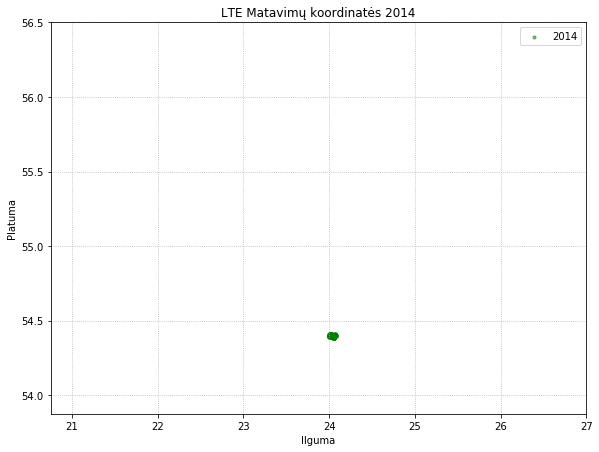
\includegraphics[scale=0.33]{img/LTE-1}
	\caption{LTE Matavimai 2014 metais. Viso – 232 matavimai}
	\label{img:LTE-1}
\end{figure}
\begin{figure}[H]
	\centering
	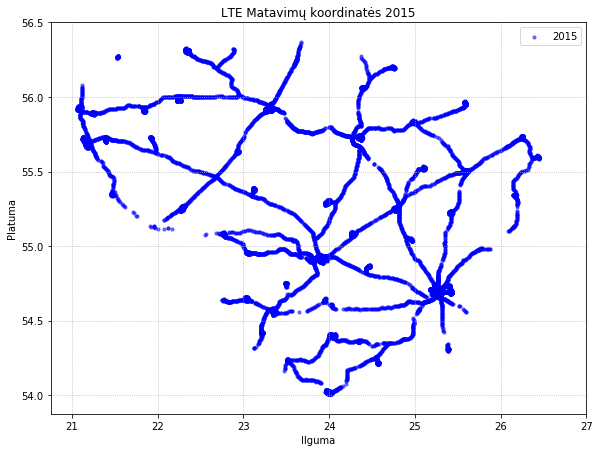
\includegraphics[scale=0.33]{img/LTE-2}
	\caption{LTE Matavimai 2015 metais. Viso – 13962 matavimai}
	\label{img:LTE-2}
\end{figure}
\begin{figure}[H]
	\centering
	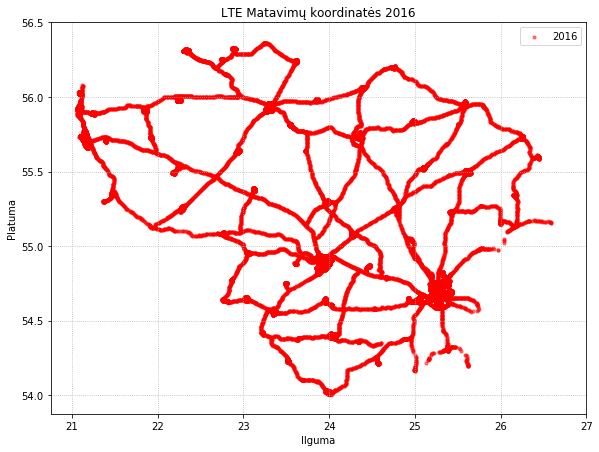
\includegraphics[scale=0.33]{img/LTE-3}
	\caption{LTE Matavimai 2016 metais. Viso – 40738 matavimai}
	\label{img:LTE-3}
\end{figure}
\begin{figure}[H]
	\centering
	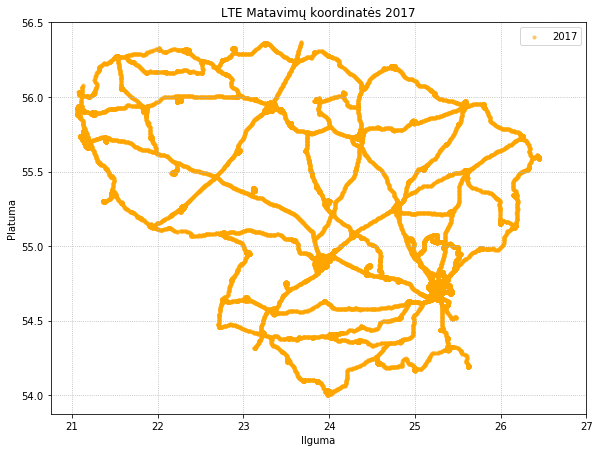
\includegraphics[scale=0.33]{img/LTE-4}
	\caption{LTE Matavimai 2017 metais. Viso – 49672 matavimai}
	\label{img:LTE-4}
\end{figure}
\begin{figure}[H]
	\centering
	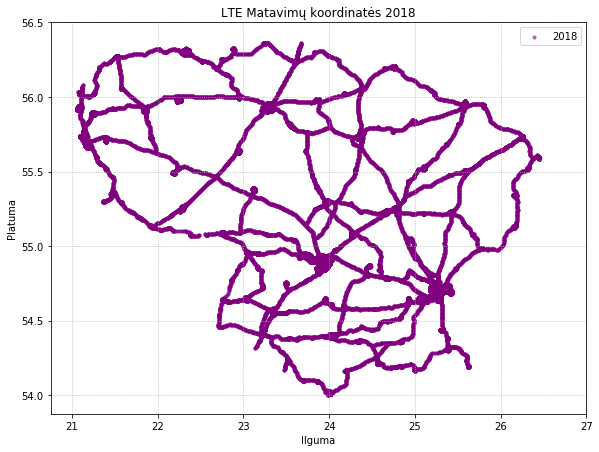
\includegraphics[scale=0.33]{img/LTE-5}
	\caption{LTE Matavimai 2018 metais. Viso – 52918 matavimai}
	\label{img:LTE-5}
\end{figure}
IPSS \textbf{WiMAX} ryšio technologijos matavimai 2014–2018 metais. Viso 18166 įrašai.
\begin{figure}[H]
	\centering
	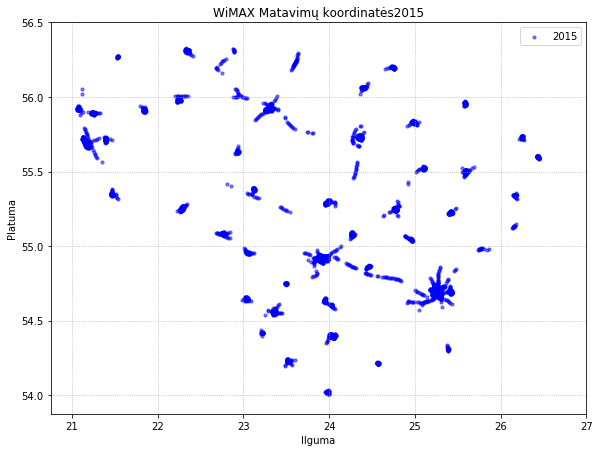
\includegraphics[scale=0.33]{img/WiMAX-1}
	\caption{WiMAX Matavimai 2015 metais. Viso – 4307 matavimai}
	\label{img:WiMAX-1}
\end{figure}
\begin{figure}[H]
	\centering
	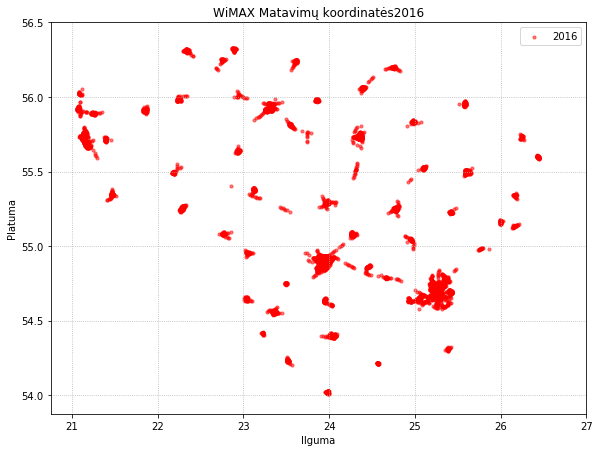
\includegraphics[scale=0.33]{img/WiMAX-2}
	\caption{WiMAX Matavimai 2016 metais. Viso – 7653 matavimai}
	\label{img:WiMAX-2}
\end{figure}
\begin{figure}[H]
	\centering
	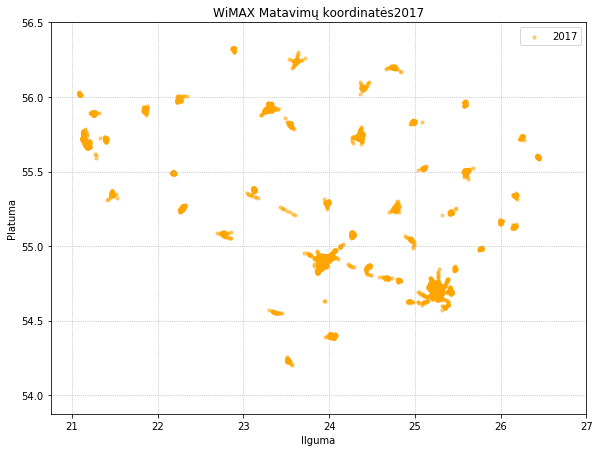
\includegraphics[scale=0.33]{img/WiMAX-3}
	\caption{WiMAX Matavimai 2017 metais. Viso – 6206 matavimai}
	\label{img:WiMAX-3}
\end{figure}

\section{Pradinių IPSS CSV failų apdorojimo „Python“ skriptas} \label{script1}
„Python“ skriptas skirtas iš duotųjų IPSS duomenų CSV failų atrinkti nereikalingus laukus ir pervadinti lietuviškus antraštės pavadinimus į vieno žodžio (vienos simbolių eilutės) angliškus pavadinimus bei sugeneruoti naujus CSV failus:
\lstinputlisting[language=Python]{scripts/script1.py}

\section{Atrinktų IPSS CSV failų duomenų papildymo „Python“ skriptas} \label{script2}
„Python“ skriptas skirtas jau atrinktiems CSV failams pridėti papildomus laukus: aukščio virš jūros lygio (gaunamas iš koordinačių), suapvalintų koordinačių reikšmių bei suapvalintos aukščio reikšmės. Šiems duomenims yra sugeneruojamas nauji CSV failai:
\lstinputlisting[language=Python]{scripts/script2.py}



\section{Eksperimentinio palyginimo rezultatai}
% tablesgenerator.com - converts calculators (e.g. excel) tables to LaTeX
\begin{table}[H]\footnotesize
	\centering
	\caption{Lentelės pavyzdys}
	{\begin{tabular}{|l|c|c|} \hline
			Algoritmas & $\bar{x}$ & $\sigma^{2}$ \\
			\hline
			Algoritmas A  & 1.6335    & 0.5584       \\
			Algoritmas B  & 1.7395    & 0.5647       \\
			\hline
	\end{tabular}}
	\label{tab:table example}
\end{table}

\end{document}

			Algoritmas & $\bar{x}$ & $\sigma^{2}$ \\
			\hline
			Algoritmas A  & 1.6335    & 0.5584       \\
			Algoritmas B  & 1.7395    & 0.5647       \\
			\hline
	\end{tabular}}
	\label{tab:table example}
\end{table}

\end{document}
